
\typeout{IJCAI-11 Instructions for Authors}

% These are the instructions for authors for IJCAI-11.
% They are the same as the ones for IJCAI-07 with superficial wording
%   changes only.

\documentclass[dvipsnames]{article}
% The file ijcai11.sty is the style file for IJCAI-11 (same as ijcai07.sty).
\usepackage{ijcai11}
\usepackage{plantuml}
\usepackage[OT1]{fontenc}
\usepackage[utf8]{inputenc}
\usepackage{minted}
\usepackage{biblatex}
\addbibresource{../bib/ijcai11.bib}

\usepackage{times}

% the following package is optional:
\usepackage{latexsym}

\usepackage{amssymb}
\newif\ifshowcomments
\showcommentstrue
%\showcommentsfalse

\ifshowcomments
\newcommand{\mynote}[2]{\fbox{\bfseries\sffamily\scriptsize{#1}}
 {\small$\blacktriangleright$\textsf{\emph{#2}}$\blacktriangleleft$}}
%\newcommand{\mynote}[2]{}
\else
\newcommand{\mynote}[2]{}
\fi
\newcommand{\comm}[1]{\mynote{Comment}{#1}}
\newcommand{\csk}[1]{\textcolor{Blue}{\mynote{Karthik}{#1}}}
\newcommand{\nick}[1]{\textcolor{Red}{\mynote{Nick}{#1}}}
\newcommand{\np}[1]{\textcolor{Green}{\mynote{Nico}{#1}}}


\newif\iflspCommEx% <lspCommEx>
\newif\ifvsceArch% <vsceArch>
\newif\ifdaGdb% <daGdb>
\newif\ifmnProb% <mnProb>
\newif\ifsolMnProb% </solMnProb>
\newif\ifsolDbg% </solDbg>
\newif\ifiro% </iro>
\newif\ifauto% </auto>
\newif\ifmyc% </myc>
\newif\ifmycext% </mycext>
\newcommand{\loadFig}[1]{{% \inputbetweentag{<tag>}{<filename>}
  \expandafter\let\csname if#1\endcsname\iftrue% Make "tag" true
  %Figure file
% dont use _ or whitespace in tags
% every tag added here be sure to add into figtag.tex

\iflspCommEx% <lspCommEx>
\begin{figure}
    \begin{plantuml}
      @startuml
      skinparam defaultTextAlignment center
      skinparam SequenceMessageAlign center
      actor User
      participant DevTool
      participant LangServer
      activate User
      activate DevTool
      activate LangServer
      User -> DevTool: open document
      DevTool -> LangServer: Notification: textDocument/didOpen; Params: document
      User -> DevTool: edit document
      DevTool -> LangServer: Notification: textDocument/didChange; Params: {documentURI, changes}
      LangServer -> DevTool: Notification: textDocument/publishDiagnostics; Params: Diagnostic[]
      User -> DevTool: execute goto definition
      DevTool -> LangServer: Request: textDocument/definition; Params: {documentURI, position}
      LangServer -> DevTool: Response: textDocument/definition; Result: Location
      User -> DevTool: close document
      DevTool -> LangServer: Notification: textDocument/didClose; Params: documentURI
      deactivate LangServer
      deactivate DevTool
      deactivate User
      @enduml
    \end{plantuml}
    \caption{Example of communication between the LSP client and server \cite{lsp}}
    \label{lspCommEx}
\end{figure}
\fi% </lspCommEx>

\ifvsceArch% <vsceArch>
\begin{figure}
    \begin{plantuml}
      @startuml
      skinparam defaultTextAlignment center
      skinparam SequenceMessageAlign center
      skinparam linetype ortho
      left to right direction
        rectangle "VS Code" {
        rectangle "Extension Host" {
        rectangle hlc [
        HTML Language Client
        ]
        rectangle plc [
        PHP Language Client
        ]
        }
        }
        
        rectangle hls [
        HTML Language Server
        ]
        rectangle pls [
        PHP Language Server
        ]
        
        hlc --> hls
        hls --> hlc: LSP over JSON-RPC
        plc --> pls
        pls --> plc: LSP over JSON-RPC
      @enduml
    \end{plantuml}
    \caption{Integration of extension into VSCode\cite{vsclspextman}}
    \label{vsceArch}
\end{figure}
\fi% </vsceArch>

\ifdaGdb% <daGdb>
\begin{figure}
    \begin{plantuml}
    @startuml
      skinparam defaultTextAlignment center
      skinparam SequenceMessageAlign center
      actor User
      participant DevTool
      participant DebugAdapter
      participant Debugger
      User -> DevTool : start debugging
      activate DevTool
      DevTool -> DebugAdapter: start debug adapter
      activate DebugAdapter
      DevTool -> DebugAdapter: initialize request
      DebugAdapter -> Debugger: start gdb
      activate Debugger
      DebugAdapter -> DevTool: response: capabilities
      DebugAdapter --> DevTool: initalized event
      User -> DevTool : set breakpoint
      DevTool -> DebugAdapter: setBreakpoints request
      DebugAdapter -> Debugger: break "hello.c:main:4"
      DebugAdapter -> DevTool: response: breakpoints
      User -> DevTool : run
      DevTool -> DebugAdapter: launch request
      DebugAdapter -> Debugger: file "a.out"
      DebugAdapter -> Debugger: run
      DebugAdapter -> DevTool: response: status
      deactivate DevTool
      deactivate DebugAdapter
      deactivate Debugger
    @enduml
    \end{plantuml}
    \caption{Example of communication between IDE's generic debugger and GDB via Debug adapter \cite{dap}}
    \label{daGdb}
\end{figure}
\fi% </daGdb>

\ifmnProb% </mnProb>
\begin{figure}
    \begin{plantuml}
      @startuml
      skinparam defaultTextAlignment center
      skinparam linetype polyline
      left to right direction
      rectangle Languages {
        usecase "JS" as js
        usecase "Python" as py
        usecase "Java" as jav
      }
      rectangle IDEs {
        usecase "VSCode" as vsc
        usecase "Eclipse" as ec
        usecase "Vim" as vim
      }
      js --> vsc
      js --> ec
      js --> vim
      py --> vsc
      py --> ec
      py --> vim
      jav --> vsc
      jav --> ec
      jav --> vim
      @enduml
    \end{plantuml}
    \caption{The {\it m+n} problem\cite{vsclspextman}}
    \label{mnProb}
\end{figure}
\fi% </mnProb>

\ifsolMnProb% </solMnProb>
\begin{figure}
    \begin{plantuml}
      @startuml
      skinparam defaultTextAlignment center
      left to right direction
      rectangle LSP_Server {
        usecase "JS" as js
        usecase "Python" as py
        usecase "Java" as jav
      }
      rectangle LSP
      rectangle LSP_Client {
        usecase "VSCode" as vsc
        usecase "Eclipse" as ec
        usecase "Vim" as vim
      }
      js --> LSP
      py --> LSP
      jav --> LSP
      LSP --> vsc
      LSP --> ec
      LSP --> vim
      @enduml
    \end{plantuml}
    \caption{Solution to {\it m+n} problem\cite{vsclspextman}}
    \label{solMnProb}
\end{figure}
\fi% </solMnProb>

\ifsolDbg% </solDbg>
\begin{figure}
    \begin{plantuml}
      @startuml
      skinparam defaultTextAlignment center
      left to right direction
      rectangle "IDE (with Generic Debugger)" {
        usecase "VSCode" as vsc
        usecase "Eclipse" as ec
        usecase "Vim" as vim
      }
      rectangle DA
      rectangle JS_DA
      rectangle Python_DA
      rectangle Java_DA
      rectangle JS_Debugger
      rectangle Python_Debugger
      rectangle Java_Debugger
      vsc --> DA
      ec --> DA
      vim --> DA
      DA --> JS_DA
      DA --> Python_DA
      DA --> Java_DA
      JS_DA --> JS_Debugger 
      Python_DA --> Python_Debugger
      Java_DA --> Java_Debugger
      @enduml
    \end{plantuml}
    \caption{Solution for debugging support\cite{dap}}
    \label{solDbg}
\end{figure}
\fi% </solDbg>

\ifiro% </iro>
\begin{figure}
    \begin{plantuml}
      @startuml
      skinparam defaultTextAlignment center
      left to right direction
      rectangle IRO
      rectangle "Format" {
        usecase "Texmate" as tm
        usecase "Atom" as at
        usecase "Ace" as ace
        usecase "Sublime3" as sub3
      }
      rectangle "Users" {
        usecase "VSCode" as vsc
        usecase "Eclipse" as ec
        usecase "Github" as gh
        usecase "Atom editor" as atsh
        usecase "Ace editor" as acesh
        usecase "Sublime editor" as sub3sh
      }
      IRO --> tm
      IRO --> at
      IRO --> ace
      IRO --> sub3
      tm --> vsc
      tm --> ec
      tm --> gh
      at --> gh
      at --> atsh
      ace --> acesh
      sub3 --> sub3sh
      @enduml
    \end{plantuml}
    \caption{{\it IRO}\cite{iro} and supported grammar formats}
    \label{iro}
\end{figure}
\fi% </iro>

\ifauto% </auto>
\begin{figure}
    \begin{plantuml}
      @startuml
      skinparam defaultTextAlignment center
      package "Template project" as TPrj {
        [LSP Client with entry points]
        [LSP Server with entry points]
      }
      file "Entry point list YAML file" as EPY
      file "Language Configuration YAML file" as LCY
      rectangle "Automation script" {
      database "Automation script module" as AutoMod
      package "LSP project" as LSPrj {
        [LSP Client]
        [LSP Server]
      }
      database "npm installer" as npi
      package "Precompiled LSP project" as LSPPrj {
        [LSP Client]
        [LSP Server]
        [npm modules]
      }
      database "VSCE" as vsce
      }
      folder "LSP Extension" as LSPex  
      TPrj --> AutoMod
      EPY --> AutoMod
      LCY --> AutoMod
      AutoMod --> LSPrj
      LSPrj --> npi
      npi --> LSPPrj
      LSPPrj --> vsce
      vsce --> LSPex
      @enduml
    \end{plantuml}
    \caption{Automation of generation of LSP extension}
    \label{auto}
  \end{figure}
\fi% </auto>

\ifmyc% </myc>
\begin{figure}
    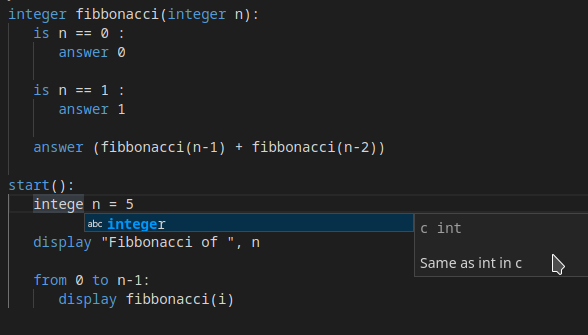
\includegraphics[width=\linewidth]{../fig/myc.png}
    \caption{Keyword syntax Highlighting, auto completion and inline documentation}
    \label{myc}
\end{figure}
\fi% </myc>

\ifmycext% </mycext>
\begin{figure}
    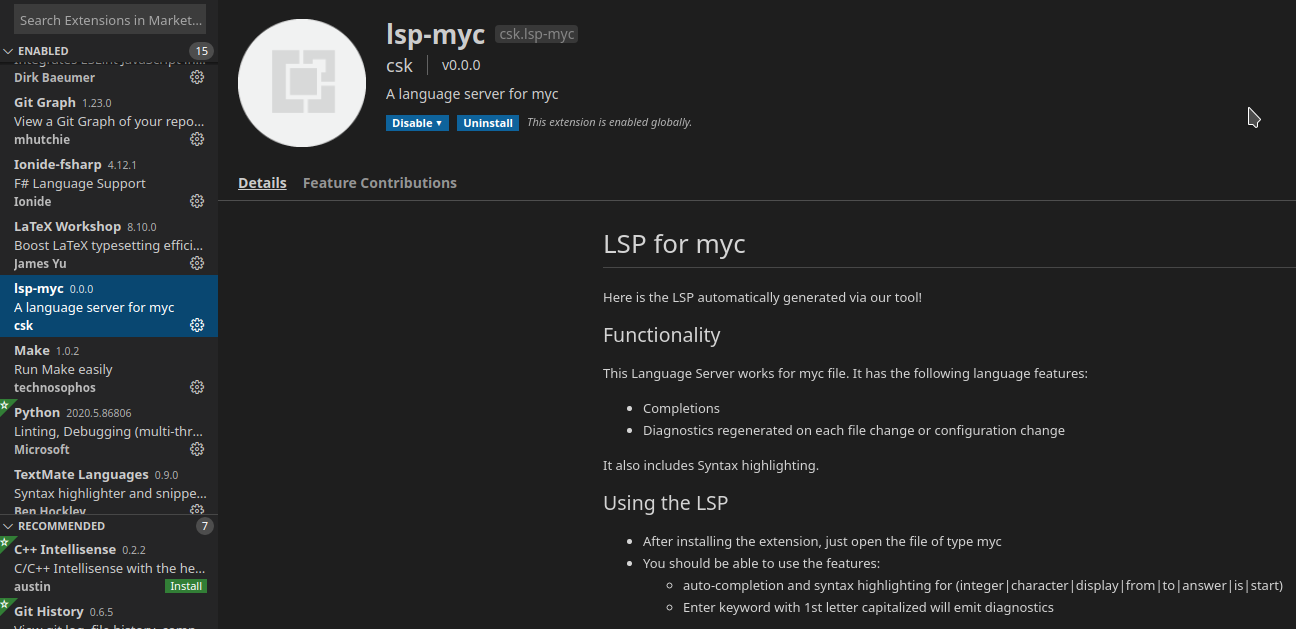
\includegraphics[width=\linewidth]{../fig/mycext.png}
    \caption{Extension for LSP of {\it myc} installed in VSCode}
    \label{mycext}
\end{figure}
\fi% </mycext>}
}% Input file

% Following comment is from ijcai97-submit.tex:
% The preparation of these files was supported by Schlumberger Palo Alto
% Research, AT\&T Bell Laboratories, and Morgan Kaufmann Publishers.
% Shirley Jowell, of Morgan Kaufmann Publishers, and Peter F.
% Patel-Schneider, of AT\&T Bell Laboratories collaborated on their
% preparation.

% These instructions can be modified and used in other conferences as long
% as credit to the authors and supporting agencies is retained, this notice
% is not changed, and further modification or reuse is not restricted.
% Neither Shirley Jowell nor Peter F. Patel-Schneider can be listed as
% contacts for providing assistance without their prior permission.

% To use for other conferences, change references to files and the
% conference appropriate and use other authors, contacts, publishers, and
% organizations.
% Also change the deadline and address for returning papers and the length and
% page charge instructions.
% Put where the files are available in the appropriate places.

\title{Generalized Source to Source Tool Support v1.2}
\author{CHAKKA Karthik Subramanyam \\ 
MOSIG-M1, ENSIMAG\\
Grenoble, France \\
karthik-subramanyam.chakka@grenoble-inp.org \\
\\
Supervised by: Nick Papoulias and Nicolas Palix} % Mosig student

\begin{document}

\maketitle

{% Mosig student
  {\hbox to0pt{\vbox{\baselineskip=10dd\hrule\hbox
to\hsize{\vrule\kern3pt\vbox{\kern3pt
\hbox{{\small I understand what plagiarism entails and I declare that this report }}
\hbox{{\small is my own, original work. }}
\hbox{{\small Name, date and signature:} Karthik, 12-06-20, }
\kern3pt
}\hfil%\kern3pt
\vrule
}\hrule}
}}
}


\begin{abstract}
  For development of source to source transpilers, though several language workbenches\cite{langworkbenches} exist, they are tied to various specificities of their environments and platforms.
  For general purpose languages, however various solutions like Language Server Protocol and Debugger Adapter Protocol exists so ensure tooling support without getting tied to specific IDE or platform.
  In this internship, applicability of Language Server Protocol and Debugger Adapter Protocol to DSLs and transpilers is investigated.
  We then propose an automation process for the tooling support and provide the prototype implementation for VSCode.
\end{abstract}


\section{Introduction}

In the development of tooling for general purpose languages, thanks to protocols such as the Language Server Protocol and the Debugger Adapter Protocol language tools are not tightly coupled to IDE/environment/platform. 
Hence, developers of programming languages can easily integrate the language support across IDEs with less effort.
For DSLs and transpilers\cite{dslbook}, there doesn't exist a generic solution to prevent coupling of tools and IDEs.
Hence, we explore the applicability of the LSP and DAP to DSLs and transpilers.
Along with the exploration, we provide a generalized process for automation of language tooling support with features such as:
\begin{itemize}
\item Language support
\begin{itemize}
  \item Code completion
  \item Syntax highlighting
  \item Inline documentation
  \item Diagnostic reporting
  \item Retrieve code documentation, etc.
\end{itemize} 
\item Debug Support
\begin{itemize}
  \item Customized project skeleton to kickstart the development of debug adapter
\end{itemize} 
\end{itemize}

\subsection{Language Sever Protocol(LSP)}
The programming language developer provides a language server and a part of the IDE(extension/plugin/module/text-editor) will act as a LSP client to obtain the diagnostics and updates the text editor accordingly.
LSP uses {\textit JSON-RPC} to communicate in order to support various features\footnote{Syntax highlighting is not yet supported by LSP. Textmate grammar is a popular solution adapted by various IDE vendors.} for a programming language such as:
\begin{itemize}
\item Code completion
\item Code navigation
\item Code snippets
\item Find references
\item Retrieve code documentation, etc.
\end{itemize}

\loadFig{lspCommEx}

The language server and client is integrated into IDE using IDE's plugin support.
Normally, the LSP server is launched by the LSP client and the initialization sequence starts during which the client is informed of the server's capabilities.
Depending on the IDE, the LSP client is launched either when user opens a project of a particular language or when the user opens a file with a particular extension that belongs to that language.
Figure \ref{lspCommEx} illustrates the communication between LSP client and server.
The communication is predominantly of 2 types:
\begin{itemize}
  \item notifications upon an event(file open, file close etc.)
  \item request-response
\end{itemize}

Having a plugin based architecture to extend the features of an IDE provides several benefits:
\begin{itemize}
  \item It frees the core IDE code from details and specific logic by transferring such burden on extensions
  \item It provides a slimmer and easy to maintain architecture for the IDE developers
  \item With good documentation and infrastructure for the extension development, huge diversity of developers from various domains can participate to make IDE and tools accessible to their respective user bases.
  \item A common testing and profiling infrastructure can be put in place to ensure testability of extensions
  \item The burden of ensuring compatibility of a toolchain is now on the plugin developer rather than IDE developer. Hence, users have lesser risk of encountering compatibility issues which is a huge problem with legacy toolchain.
\end{itemize}

\subsection{Debugger Adapter Protocol(DAP)}
Ideally, debuggers can also take the same route as language compilers i.e. have a debugger server that communicates with IDE's text editor.
But, this adaptation requires relatively more effort and it's highly unlikely that programming language developers will adapt it anytime soon.
Hence, Microsoft proposes the Debugger adapter protocol.
It defines how an IDE with a generic debugger executes language specific debugging features via a wrapper called debugger adapter.
This wrapper makes it possible to decouple language specific debugger and IDE.
Language developers will need to write an adapter to their language's debugger that communicates with IDE's generic debugger.
The generic debugger and debug adapter uses {\textit JSON} format, based on an obsolete {\textit V8} Debugging Protocol\footnote{Current DAP is at v1.4. At v2.0, it's expected to adapt JSON-RPC like LSP.}, to support various features for debugging code such as:
\begin{itemize}
\item Addition and deletion of different types of breakpoints
\item Inspection of variables and symbols
\item Inspection of memory
\item Call stack
\item Stack information, etc.
\end{itemize}

\loadFig{daGdb}

The debugger adapter is integrated into IDE using IDE's plugin support.\footnote{Very often, the language server/compiler and Debugger adapter + Debugger are packed into one language support plugin/extension.}
Figure \ref{daGdb} shows an example where an IDE uses of gdb as the debugger using debug adapter. The generic debugger of IDE issues commands via requests.
The debugger adapter is responsible to convert this command to gdb command, for example "setBreakpoint" request from generic debugger is converted to "break file:line" gdb command by debugger adapter.

\section{Problem Statement and Related Work}
Growth and utility of any programming language, no matter how well designed it is, is significantly determined by it's popularity i.e. the strength and diversity of it's user-base.
Modern IDEs support multiple languages and several language-based features.
This poses a new problem to the developers of compilers of programming languages.
Since, the users tend to prefer languages that are 'well-supported' within their favorite IDEs, the developers of new programming languages are left with herculean task of implementing language support features for their language using the SDKs provided by IDE vendors for multiple popular IDEs.
This {\textit m+n} problem is shown in the fig \ref{mnProb}.
Moreover, for the IDE vendor, it's complex to maintain and evaluate each integration without compromising on performance/security of the IDE architecture.
Also, since language developers tend to prefer popular IDEs, it's difficult for new IDEs to become more accepted and used as well.

\loadFig{mnProb}

To address above issues, Microsoft introduced Language Server Protocol and Debugger Adapter Protocol.

Figure \ref{solMnProb} shows how LSP can provide a solution to {\textit m+n} problem.
\loadFig{solMnProb}

Figure \ref{solDbg} shows the use of generic debugger and debug adapters to provide support for various languages.
\loadFig{solDbg}

Using these protocols, any language developer can easily build a language server and debugger adapter which can be integrated with multiple IDEs(as plugins) with minimal effort.
In the process, the development of languages is democratized.
New languages, backed by independent passionate community of developers can compete on an even level with languages backed by multi-national corporations.
Even though the problem is solved in the development of languages, the sub-domain of DSLs and transpilers still face the same challenges of pre-LSP and pre-DAP era.

\section{Proposed Solution}
In theory, it is possible to exploit LSP and DAP for providing support for transpilers.
This internship investigates, via experimentation, how feasible is it to directly use or adapt the existing solutions and framework based on LSP and DAP for transpilers.

\subsection{Using LSP for Transpiled languages}

Means to provide the standard programming language features to a DSL that gets transpiled to a known language is explored.
A series of realistic examples of targeted DSLs is explored, with the eventual goal of supporting DSLs developed by the ERODS team targeting the Linux Kernel.

In this context, the features are independent of the transpiled/target language, hence, it is equivalent to implementing a new language server for the source language i.e. the DSL.

Implementation wise several features are dependent on static data from language specification(keywords, literals, tokens etc.).
Hence, by using scripting to strategically replace various points in code dealing with static language data related to a certain feature, we can generate a working project.
By scripting shell commands used for generation of plugin from project, we can automate end to end, i.e. from projection generation to plugin creation.

\subsection{Using DAP for Transpiled languages}

The goal is to see how we can translate the features of DSL's target language's debugger(gdb in this case), for debugging in source DSL language.
For example, how to translate a breakpoint in source DSL, to target language executable so that it can be interpreted by target language's debugger.

To achieve this, we investigate feasibility of using DAP to integrate into VSCode a wrapper for DA of gdb which performs the above mentioned translation.

Implementation wise several features are dependent on the target language debugger.
Hence, the scope of automation is limited in comparison to language support.
However, the architecture and base code will remain same with few constant values.
By scripting we can supply these constants and automate project generation.

\section{Experimentation}

For experimentation there are several LSP frameworks available, which allow us to implement Language server in various languages.
Ample documentation, heavily commented code examples and strong online community, were the motivating factors for us to choose VSCode with it's extension development framework in Typescript language to perform our experiments.

\subsection{Understanding architecture of VSCode}
Though the LSP and DAP decouples IDE from language tools and eliminates major effort, for the implementation/experimentation it's essential to understand the plugin architecture of the test environment(VSCode in our case).
Hence, as an exploratory work, we had to create a simple "Hello World" extension project and understand how to run and debug it.
Normally, the core of the extension is launched as a separate process and it configures and communicates with VSCode via well-defined contribution points and communication apis respectively.
Figure \ref{vsceArch} demonstrates how LSP plugins are integrated with VSCode.

\loadFig{vsceArch}

The plugin can be configured to launch on an action(ex: shortcut key press)/on opening a file etc.
This method of invoking and running extensions provides several advantages:
\begin{itemize}
\item It abstracts low level details such as memory, and concurrency management, etc. from developers. Hence, even amateur developers can build extensions.
\item Allows building a robust code and protects the core architecture from security vulnerabilities arising out of extensions
\item Since extension is running in separate process, IDE can remain independent of the resource consumption by extension.
\item Any security issues in extension will cause OS to kill the extension process rather than whole IDE.
\end{itemize}
Also, as part of understanding the deployment, we created a package and tested it by installing the package as an extension.
Thanks to Microsoft's {\textit vsce}\cite{vsce} npm module, it's very easy to generate a package installer from a compiled extension project.

\subsection{Language Support}
To check initial feasibility, we setup toolchain, compiled and executed several simple examples.
Using lsp-sample example\cite{vsclspex}, we understood how to perform auto-completion and actions based on regular expressions.
We were able to achieve the above mentioned features for our DSL via modifying entry points\footnote{points in code which can be modified to change the behavior without impacting the general architecture/code flow} in the Extension example code.
This is independent of the AST source code of the DSL for which we aspire to build language server.

\subsubsection{Syntax highlighting}
Syntax highlighting is not supported by LSP currently.
Different IDEs use different formats.
Fortunately, there's an online tool called {\textit IRO}\cite{iro}, that defines it's own language for defining grammar and let's us generate grammar files of several formats from it.
Figure \ref{iro} indicates the diversity of grammar formats supported by IRO.

\loadFig{iro}

Textmate grammar is the most popular one and is supported by several IDEs.
Textmate grammar files identified by {\textit tmLanguage} extension uses XML to define their syntax highlighting grammar.
It consists of a hierarchical structure of language elements which needs to defined using series of regular expressions for a hierarchy of scopes.
XML is cumbersome to write and even more difficult to validate correctness manually.
The IRO website abstracts this complexity and let's us test and debug the grammar in the portal.

For automation, we use scripting to fill in the contents of textmate grammar file across different scopes from user input.

Though there is not a standard defined for syntax highlighting as of now, a solution like IRO will cover practically almost all the popular IDEs/Text editors \cite{iroexp}.

\subsection{Debugging Support}

To understand the architecture of debug adapter, we setup a debug adapter\cite{vscdaex} that works with a debugger that inspects the contents of markdown files.

For generic debug support for transpiled languages, we can build a wrapper to debugger adapter of target language that translates source language debugging commands to those of target language.
But, for a transpiled language, in order to get better picture of debugging process, additional work needs to be done to show the link between source and target languages involved in transpilation on the GUI.

Alternatively, we can simply write our own debugger adapter that directly works with target language.
To explore this possibility further, we wrote a python script which controlled gdb.
But, integrating this as VSCode extension's debugger adapter is yet to be done.

\subsection{Automation}
During exploratory work to understand plugin architecture and experimentation with various projects to implement various features, we realized a great potential for automation.
In fact, the examples we executed, not only covers most practical use-cases but also quite extensible.
Hence, for new languages, we can strategically modify and append to examples\cite{vsceex} for developing the support for most feature set.

\subsubsection{Language Support}
We successfully automated creation of a language support extension with features such as:
\begin{itemize}
  \item Syntax highlighting for keywords.
  \item Auto-completion of keywords.
  \item Diagnostic information for words that match a regular expression. 
  \begin{itemize}
    \item In our case we publish some messages when the word entered is a 1st letter capitalized version of a keyword(in our case, all keywords are fully in lower case).
  \end{itemize} 
\end{itemize}

\loadFig{auto}

Automation is achieved as described below:
\begin{itemize}
  \item A template project is provided to automation script(written in python). This project contains:
  \begin{itemize}
    \item All the entry points in various files dealing with static information marked with keywords enclosed in special characters.
    \item Code that processes data dynamically for the entry points in various files during the run-time
  \end{itemize}
  \item The user provides YAML file which supplies the values to the keywords in the entry points in the files
  \item We have about 30 files, but the files that contains entry points are 5 files. In order to avoid having to scan all the files, we supply another YAML file listing all the files and corresponding entry points.
  \item The automation script makes it possible to supply data to both types of entry points:
  \begin{itemize}
    \item Static information: The automation script makes use of both the YAML files to identify the static entry points and supply the values by overwriting the keywords.
    \item Dynamic information: The YAML file holding all the language configuration values is converted into a JSON file and saved in the project. This is natively imported by the server and processed during run-time.
  \end{itemize}
  \item Post creation of the project from the template, it installs all the necessary npm modules which are required to compile the project
  \item {\textit vsce} npm module is used to compile the project and generate a packaged file using which we can install our lsp project as a VSCode extension.
  \item Post this the project is deleted and only the extension file remains waiting to be collected from the user.
\end{itemize}

Figure \ref{auto} summarizes the automation process

Hence, from user perspective, getting quick support for new language is a simple 3-step process:
\begin{itemize}
\item Write the language configuration YAML file. Below is an snippet from language configuration YAML of the language {\textit myc} which transpiles to C and whose syntax is inspired by python:
\begin{minted}[frame=single,linenos]{yaml}
lang_name: myc
auth: csk
ver: 0.0.0
lang_id: myc
desc: LSP automatically generated!
keywords:
  - name: integer
    det: c int
    doc: Same as int in c
  - name: character
    det: c char
    doc: Same as char in c
  - name: display
    det: c print
    doc: display output on console
  - name: from
    det: c for
    doc: for loop initialization
\end{minted}
\item Run the automation tool
\item Install the extension obtained. The screenshot of the extension installed can be seen in figure \ref{mycext}. As you can see from the screenshot in figure \ref{myc}, after installation of the extension, we get syntax highlighting, autocompletion and inline documentation for keywords in our DSL {\textit myc}
\loadFig{mycext}
\loadFig{myc}
\end{itemize}

\subsubsection{Debugging Support}
For debugging support, the debug adapter protocol lets an IDE have a generic debugger but for a transpiled language additional work has to be done in order to effectively show on the front-end, the link between source and target languages involved in transpilation in order to get better picture of what we are trying to debug.
At the moment, we do not have a generic template project like we do for language support extension.
However, we built a tool to generate a customized skeleton project which can be used by the language developers to jump start their development.

Implementation details of the automation are quite similar to the one described in previous section.
Here the only difference is that we stop after generating the project.

\section{Conclusion and Future work}
For language features of a DSL, the approach taken is not different from that of any language.
With the exception of advanced features like semantics-aware auto-completion, we were able to successfully automate creation of language support plugin by reusing entry points used by general purpose languages for several features.
An automation in this direction will enable several developers to quickly implement and test their ideas in VSCode, even before writing an actual AST.

For debugging support, additional work is required on the front-end to effectively illustrate the link between the languages.
Since, we are dealing with front-end, we risk getting tied to a specific IDE.
Pursuing in such a direction will effectively undo the benefits derived from DAP and get us bogged down to IDE specific implementation like pre-DAP era.
Hence, additional exploratory work is required to see if this can be overcome by abstraction of implementation details via another protocol.
However, there is a possibly impactful opportunity to re-use (through a middleware) the existing DAP implementations of target (general purpose) languages to debug the source DSLs.

%% The file named.bst is a bibliography style file for BibTeX 0.99c
\printbibliography
% \bibliographystyle{named}
% \bibliography{ijcai11}

\end{document}

%% Local Variables:
%% TeX-master: t
%% mode: latex
%% mode: flyspell
%% coding: utf-8
%% End:
